\section{Aprendizado em Profundidade}
\label{s.deep_learning}

\begin{frame}{Aprendizado em Profundidade}
	\begin{itemize}
		\justifying
		\item Representações de informações \textbf{sofisticadas} a partir de representações mais \textbf{simples}~\cite{Hinton:86};
		\\~\\
		\item Estruturado através de diversas \textbf{camadas} e milhares de \textbf{parâmetros};
		\\~\\
		\item Aplicado em tarefas mais \textbf{complexas} apesar de \textbf{custo computacional} mais elevado.
	\end{itemize}
\end{frame}

\begin{frame}
	\begin{figure}
		\centering
		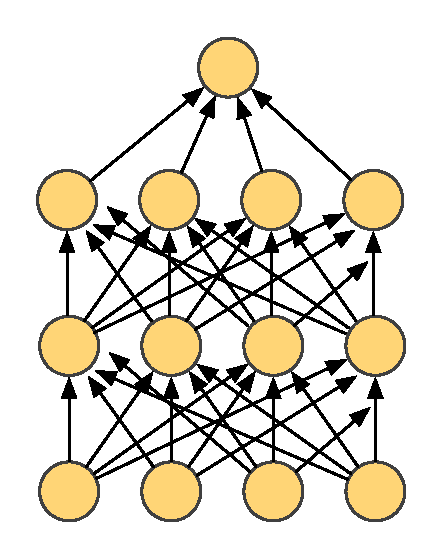
\includegraphics[scale=0.625,angle=270]{figs/nn.eps}	
		\caption{Exemplo de uma arquitetura multi-camadas de uma Rede Neural.}
		\label{f.nn}
	\end{figure}
\end{frame}

\begin{frame}
	\begin{figure}
		\centering
		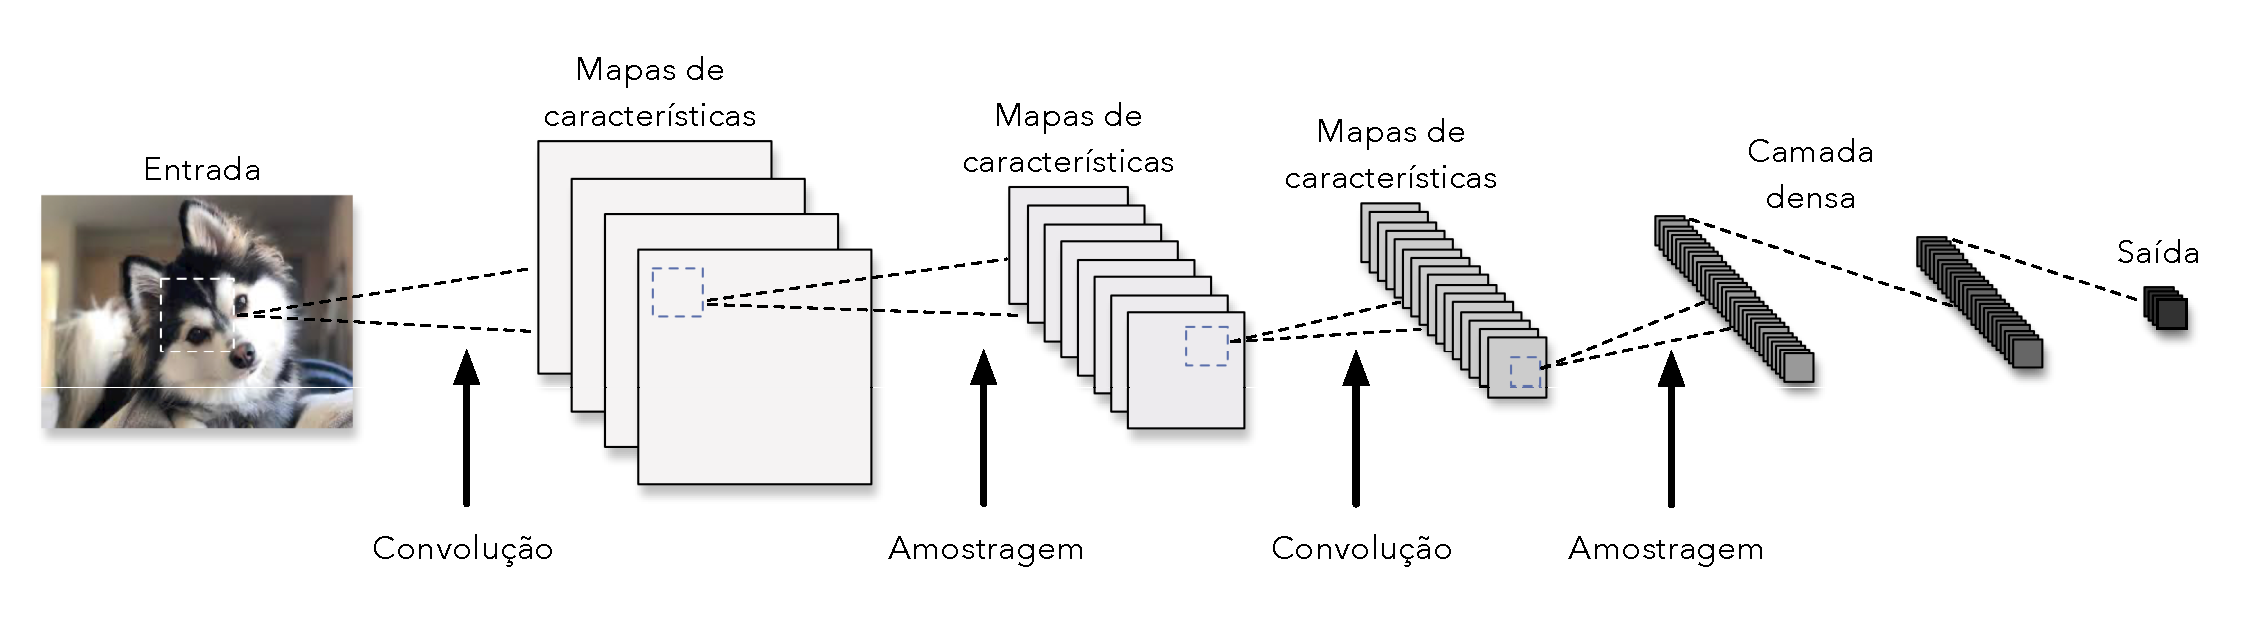
\includegraphics[scale=0.275]{figs/cnn.eps}	
		\caption{Exemplo de uma arquitetura de uma Rede Neural Convolucional.}
		\label{f.cnn}
	\end{figure}
\end{frame}

\begin{frame}
	\vspace*{0.5cm}
	\begin{figure}
		\centering
		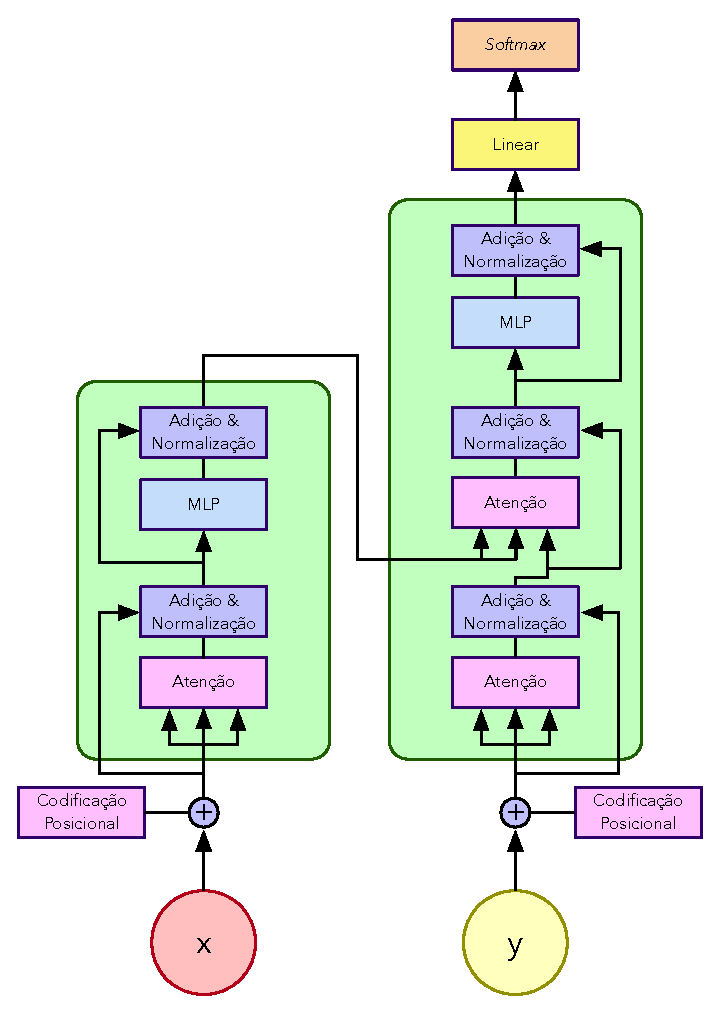
\includegraphics[scale=0.425]{figs/transformer.eps}	
		\caption{Exemplo de uma arquitetura de um Transformador.}
		\label{f.transformer}
	\end{figure}
\end{frame}